% vim:ts=4:sw=4
% Copyright (c) 2014 Casper Ti. Vector
% Public domain.

\chapter{引言}
\section{背景分析}
随着网络和移动设备普及,人们越来越多地用移动设备来进行自己的社交活动,现在层出不穷的社交类应用一直在涌现,更为显著的是wechat其生态圈已经成为了中国用户一种特定的生活模式,所以移动应用在人们社交关系中起到的作用不言而喻。

并且在这个信息爆炸时代下,由于大量的信息涌到人们眼前,而不断兴起的社交媒体更是进一步将信息碎片化。不像文字一般,照片、图像作为不易切割的单位在传递信息过程中备受用户青睐。而图片类移动社交应用因为其独特性而成为了新一代移动应用的一个热点,比如国外的instagram就是图片分享类社交的先行者。而flickr,snapchat,乃至于现在出现在中国的众多的移动社交应用都在充斥在人们的生活之中。甚至有人断言到“分享相片是社交网络的将来”。

% \begin{figure}[thbp!]
% \centering
% \begin{minipage}[t]{0.1\textwidth}
% \centering
% \includegraphics[width=1cm,height=1cm]{img/chap1/instagram.png}
% \caption{清明}
% \end{minipage}

% \begin{minipage}[t]{0.4\textwidth}
% \centering
% \includegraphics[width=1cm,height=1cm]{img/chap1/flickr.png}
% \caption{反复}
% \end{minipage}


% \begin{minipage}[t]{0.7\textwidth}
% \centering
% 
\includegraphics[width=1cm,height=1cm]{img/chap1/Snapchat.png}
% \caption{反复}
% \end{minipage}
% \end{figure}


\begin{figure}[h] 
\begin{minipage}[t]{0.3\linewidth}
\centering
\includegraphics[width=\textwidth]{img/chap1/flickr.png}
\caption{flickr \label{flickr}}
\end{minipage}
\hfill
\begin{minipage}[t]{0.3\linewidth}
\centering
\includegraphics[width=\textwidth]{img/chap1/instagram.png}
\caption{instagram\label{instagram}}
\end{minipage}
\begin{minipage}[t]{0.3\linewidth}
\centering
\includegraphics[width=1.2cm,height=1.2cm]{img/chap1/snapchat.png}
\caption{snapchat\label{snapchat}}
\end{minipage}

\end{figure}

上面的一组图展示了最近在图片分享应用中非常火热的几款应用。

其中图1.1是Flickr,是雅虎旗下图片分享网站。为一家提供免费及付费数位照片储存、分享方案之线上服务,也提供网络社群服务的平台。其重要特点就是基于社会网络的人际关系的拓展与内容的组织。而随着移动应用的兴起,其在2013年也提出了Android版本,但因为其对于移动社交市场的响应滞后性,其占到的份额已经变小。

图1.2是instagram是一款典型的图片型应用,而且最开始的专业的滤镜功能将一大帮摄影家囊括在了它的用户群之中,从而让摄影家有了扩展他们社交圈的方法,但之后由于用户的泛化,同样需要更进一步的好友推荐的方法。

图1.3是snapchat,这是一款“阅后即焚”的图片型软件,由其发送图片的时效性而著名。

总结以上图片分享社交应用,与以往社交应用类似的是大多数的图片分享社交应用要么是熟人社交圈或者弱关系社交圈。而在这种关系社交类应用中,存在着用户难以找到令他们感兴趣的用户的不足。

\begin{figure}[h] 
\begin{minipage}[t]{0.45\linewidth}
\centering
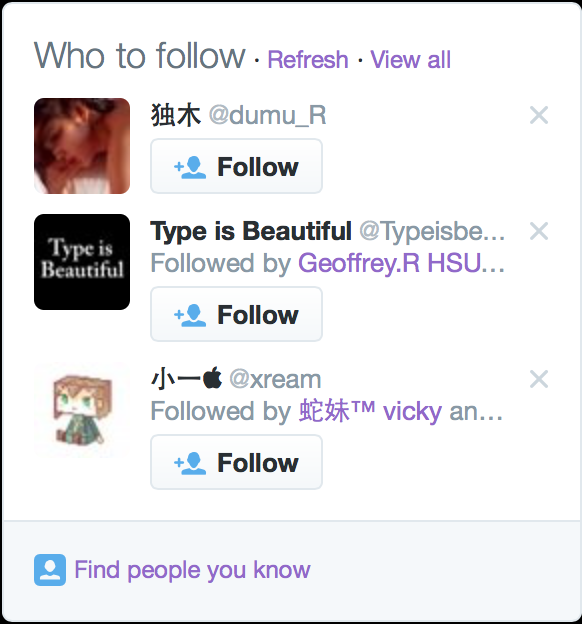
\includegraphics[width=\textwidth]{img/chap1/twitter_recommend.png}
\caption{Twitter推荐,\\根据其已关注用户的关注关系推荐\label{Twitter推荐,根据其已关注用户的关注关系推荐}}
\end{minipage}
\hfill
\begin{minipage}[t]{0.45\linewidth}
\centering
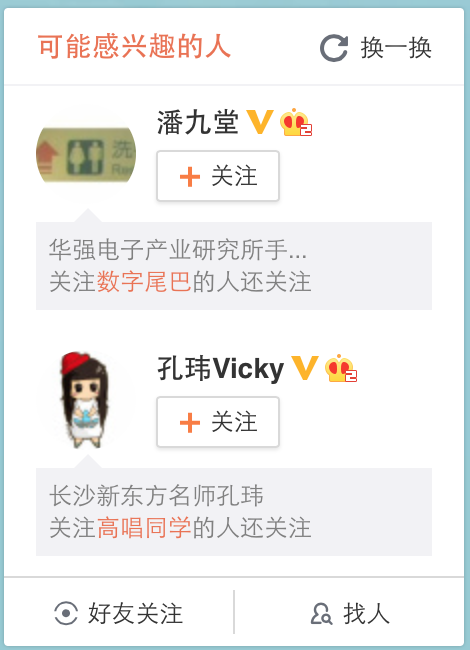
\includegraphics[width=\textwidth]{img/chap1/weibo_recommend.png}
\caption{weibo推荐,\\与twitter一样,同样由关注用户的关系所推导\label{weibo推荐,}}
\end{minipage}

\end{figure}

如今的社交应用都在尝试不同的方式帮助用户去寻找他们感兴趣的用户。比如微信的“摇一摇”、“漂流瓶”是一种具有随机性的推荐好友的方式,但除了一部分特定的人群,大部人的接受度并不高。而基于地点信息推荐的方式,很多社交应用都为用户设置了查看附近的人,但使用这项功能的人并不是很多。而基于用户的兴趣,在类似于twitter,weibo这种弱关系社交中,根据关注人的和用户的某些特性,推荐好友的功能,这给予了用户一个很好的体验。在如今的classfication中,deepwalk\parencite{deepwalk},line\parencite{node1}, node classification\parencite{node}深度学习\parencite{deep}等算法都是未来根据用户关系来分类,从而帮助用户去寻找他们感兴趣的人。


\begin{figure}[h] 
\begin{minipage}[t]{0.25\linewidth}
\centering
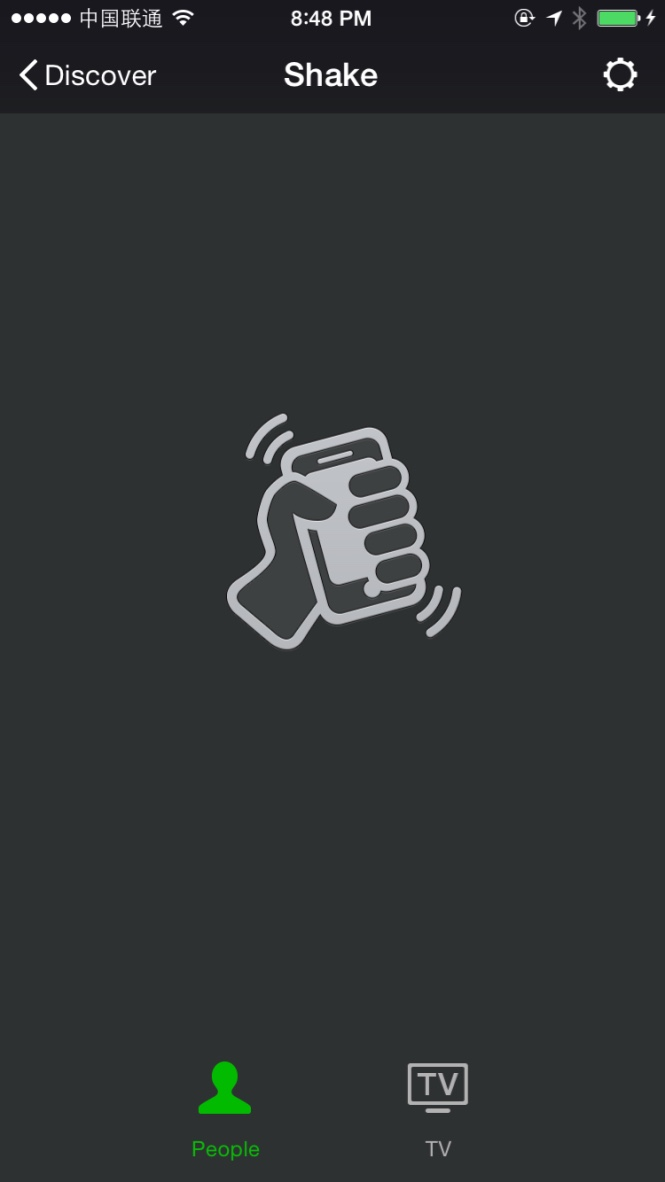
\includegraphics[width=\textwidth]{img/chap1/shake.jpg}
\caption{摇一摇\label{flickr}}
\end{minipage}
\hfill
\begin{minipage}[t]{0.25\linewidth}
\centering
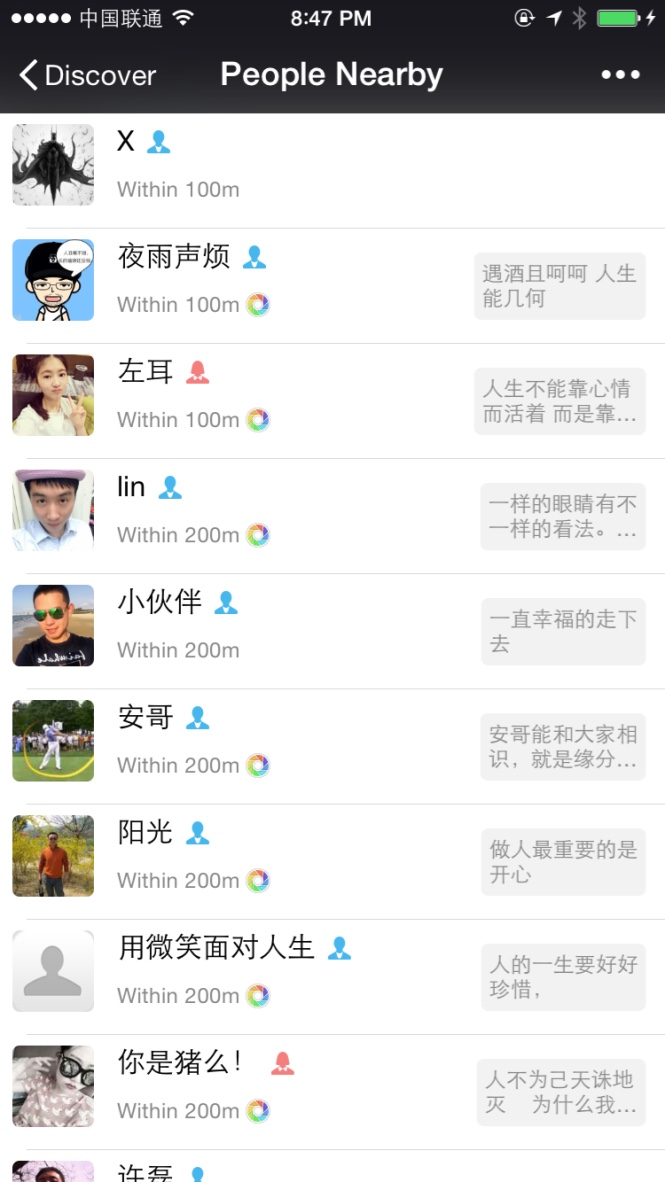
\includegraphics[width=\textwidth]{img/chap1/Nearby.jpg}
\caption{附近的人\label{instagram}}
\end{minipage}
\hfill
\begin{minipage}[t]{0.25\linewidth}
\centering
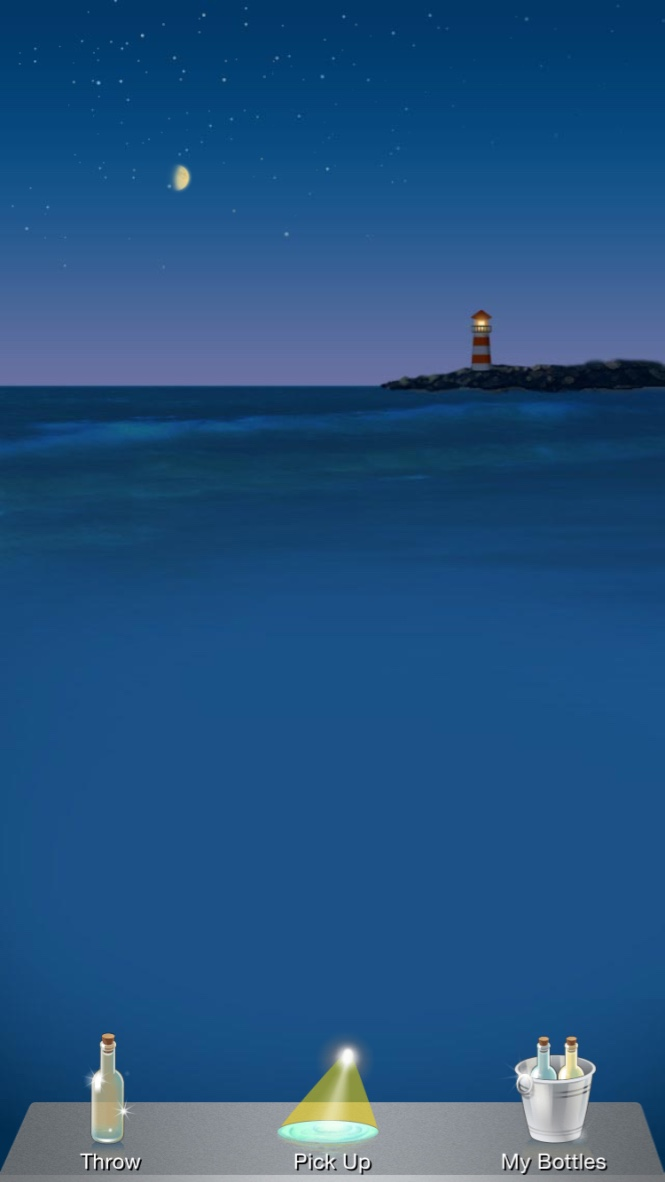
\includegraphics[width=\textwidth]{img/chap1/bottle.jpg}
\caption{漂流瓶\label{snapchat}}
\end{minipage}
\hfill
\end{figure}

上面一组图是wechat所做的各类关于增加用户好友关系的探寻。

图1.5是著名的“摇一摇”,他所做到的是利用即时性,和随机性为同时想扩展社交圈子的用户提供一个通道,但在现在中国已经成为一些人发展一些私密关系的工具。

图1.6展示的是wechat的“附近的人”,通过位置关系将可能成为朋友的人绑在了一起。

图1.7是“漂流瓶”,与“摇一摇”不同的是它是非即时的社交方式,同样是以想扩充社交圈这种意愿为纽带。

虽然现在的方式各种各样,但无可否认的是至今不存在一种很好的方式提供给用户去拓展他们的社交圈子。

这就产生了本研究的一个最初的动机:

 \textbf{能否通过一种图片交流的方式提供图片类应用的用户去认识新朋友的渠道?}

而最近由于人脸识别技术的火热,市面上不断在涌现着与人脸识别关系密切的应用,比如face++与阿里巴巴在支付宝上联合推出的“刷脸”支付功能。

这些给予了笔者以灵感,笔者拟应用人脸的特征去提供一种独特的方式给用户去拓展他们的社交圈子,结合了传统的“夫妻脸“的概念,其中最基础的方式就是以人脸相似度去实现一个应用。之后通过实验的不断调整,加入其他特征去调整最后的好友推荐算法,得出最后的适合用户的匹配好友算法。
\section{方案概述}
􏰉􏴳􏰭􏴴􏴵􏴶􏴷􏰿􏴸􏴹􏴘􏰏􏲦􏲜􏱲􏴺􏰭􏴻􏲆􏴻􏴼􏰏􏱦􏴷􏱜􏰒􏴽􏳯􏴾􏴿􏵀􏱾􏱜本文提出基于人脸识别技术的图片社交平台,利用人脸识别的技术,不但能够提高人脸识别技术的通用性,并能提高用户对于社交应用的体验。根据不同的用户脸部特征,个人信息,本文对于基于用户特征值的匹配算法的可行性进行了系统的研究。基于已有的特征值,推荐给用户各项指标都符合其标准的好友,使得可以为用户提供一个良好的方式去扩展他们的社交圈。


因此本文是对于图片社交应用的一种基于人脸识别方式的好友扩展方式的研究,基本的工作可以总结为如下:
\begin{enumerate}
\item 了解现有的社交应用给予用户的扩展好友的方式,调研相关的人脸识别的技术和算法,提出一种基于人脸特征的好友推荐匹配算法
\item 基于face++提供的api,完善在node.js平台上sdk的支持,并调研和准备应用的数据,存储到数据库中。
\item 基于angularJS+Ionic框架,开发出一款能够应用在三个移动手机平台上的应用。该应用不但能有效的解决用户好友来源的问题,并且可以在好友推荐中,为用户推荐符合用户的好友。同时,根据用户的反馈能够及时的调整对应的匹配算法。
\item 对于基于不同算法的好友推荐算法,进行实际的用户效果的测试,通过实验数据的比较取得一种较高满意度的推荐算法。实验结果表明本应用的好友推荐算法具有较高的实用价值和扩展性。
\end{enumerate}

% \section{研究的目的和意义}
\section{本文组织}
第一章包括背景和对研究的分析,及本文组织。第二章介绍论文相关技术和工作。第三章详细给出系统的设计。第四章给出系统的实现。第五章进行实验和展望。最后进行了总结。
% 中文测试文字。
% \pkuthssffaq%

